\documentclass[12pt]{article}
\frenchspacing
\usepackage[utf8x]{inputenc}
\usepackage[T2A]{fontenc}
\usepackage{amsmath}
\usepackage{amsfonts}
\usepackage{amssymb}
\usepackage[russian]{babel}
\usepackage{wrapfig}
\usepackage{graphicx}
\usepackage[left=2cm,right=2cm,top=2cm,bottom=2cm,bindingoffset=0cm]{geometry}
\author{Рашковецкий М.М., группа 526т}
\date{\today}
\title{Лабораторная работа 2.1.2\\Определение $C_p/C_v$ методом адиабатического расширения газа}
\begin{document}
	\maketitle
	
	{\parindent=1cm \hangindent=1cm \parskip=0.5cm
	{\bfseries Цель работы:} определение отношения $C_p/C_v$ для углекислого газа по измерению давления в стеклянном сосуде.
	
	\hangindent=1cm
	{\bfseries Оборудование и материалы:} стеклянный сосуд с трубками; U-образный жидкостный манометр; газгольдер с углекислым газом; секундомер.\par}
	\section*{Краткая теория}
	
	\indent Экспериментальная установка (рис. \ref{fig:scheme}) cостоит из стеклянного сосуда A (объёмом около 20 л) с краном $K_2$, и U-образного жидкостного манометра M для измерения избыточного давления газа в сосуде. Избыточное давление в сосуде создаётся путём накачивания углекислого газа из газгольдера через кран $K_1$.
	
	\begin{figure}[h!]
	\caption{Схема установки}
	\label{fig:scheme}
	\begin{center}
	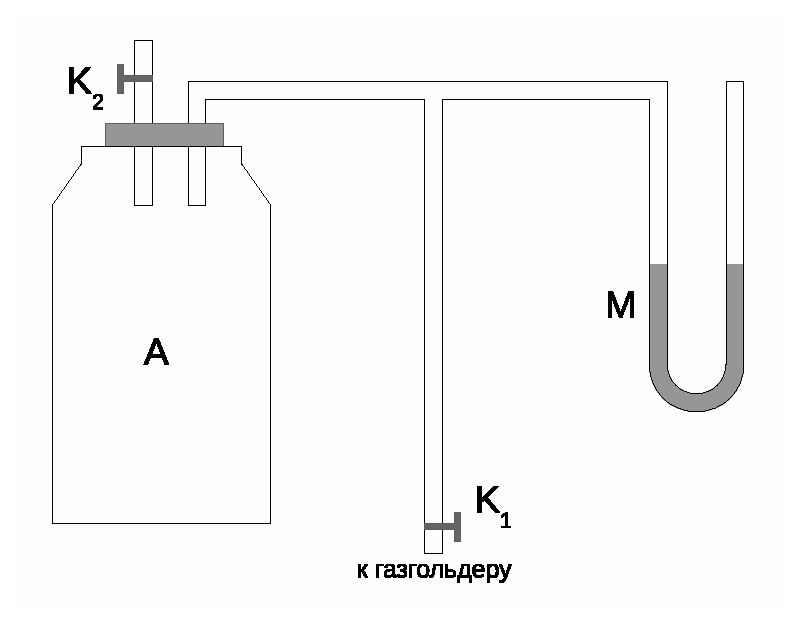
\includegraphics[scale=0.7]{scheme.eps}
	\end{center}
	\end{figure}
	
	Схематические графики процессов, происходящих с газом, показаны на рис. \ref{fig:process}. Штриховой линией показаны изотермы. При накачивании газ несколько нагревается, но спустя некоторое время остывает ($1 \rightarrow 2$), так что в начале опыта в сосуде A находится исследуемый газ при комнатной температуре $T_0$ и давление $P_1$ немного больше атмосферного $P_0$:
	\begin{equation}
	\label{eq:pressure_base_1}
	P_1=P_0+\rho g\Delta h_1.
	\end{equation}
	
	\begin{figure}[h!]
	\caption{Графики процессов}
	\label{fig:process}
	\begin{center}
	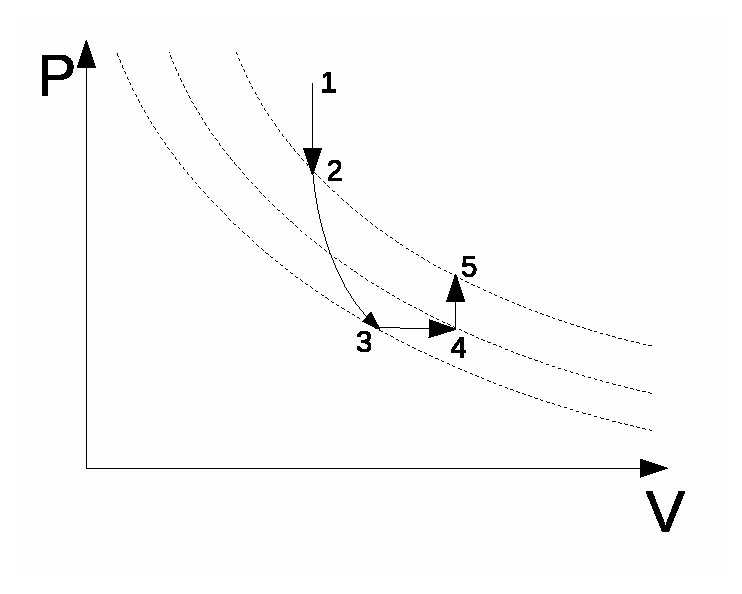
\includegraphics[scale=1]{process.eps}
	\end{center}
	\end{figure}
	
	После открытия крана K, соединяющего сосуд A с атмосферой, давление и температура газа будет понижаться сначала адиабатически в течение $\Delta t \sim 0{,}5 \,\text{с}$ ($2 \rightarrow 3$), а потом идёт изобарное расширение ($3 \rightarrow 4$). После закрытия $K_2$ газ изохорически нагревается до комнатной температуры ($4 \rightarrow 5$), давление повышается до
	\begin{equation}
	\label{eq:pressure_base_2}
	P_2=P_0+\rho g\Delta h_2.
	\end{equation}
	
	Исследуем зависимость соотношения перепадов давлений $\frac{\Delta P_1}{\Delta P_2}$ от времени открытия клапана $\tau$.
	
	Можно достаточно точно считать газ идеальным. Рассмотрим изобарное расширения, записав уравнение теплового баланса для изменяющейся со временем
	\begin{equation}
	\label{eq:ch_mass}
	m = \mu \frac{P_0 V_0}{RT}
	\end{equation}
	массы газа:
	\begin{equation}
	\label{eq:heat_balance_base}
	C_P m dT = - \alpha \left( T-T_0 \right) dt,
	\end{equation}
	где $C_P$ --- удельная теплоёмкость при постоянном давлении, а $\alpha$ --- положительный коэффициент, характеризующий теплообмен, $V_0$ --- объём сосуда.
	
	\begin{equation}
	\label{eq:heat_balance2}
	C_P \mu \frac{P_0 V_0}{RT} dT = - \alpha \left( T-T_0 \right) dt,
	\end{equation}
	или
	\begin{equation}
	\label{eq:heat_balance_diff_eq_base}
	\frac{dT}{T \left( T-T_0 \right)} = -\frac{\alpha R dt}{C_P P_0 V_0 \mu}.
	\end{equation}
	
	Поскольку
	\begin{equation}
	\label{eq:temp_other_form}
	\frac{1}{T \left( T-T_0 \right)} = - \frac{1}{T_0} \left( \frac{1}{T} - \frac{1}{T-T_0} \right),
	\end{equation}
	получаем
	\begin{equation}
	\label{eq:heat_balance_diff_eq2}
	\frac{dT}{T_0} \left( \frac{1}{T} - \frac{1}{T-T_0} \right) = \frac{\alpha dt}{C_P m_0 T_0}.
	\end{equation}
	
	Сократим на $T_0$:
	\begin{equation}
	\label{eq:heat_balance_diff_eq_final}
	\frac{dT}{T} - \frac{dT}{T-T_0} = \frac{\alpha dt}{C_P m_0},
	\end{equation}
	проинтегрируем и получим
	\begin{equation}
	\label{eq:heat_balance_eq_integr}
	\ln \left( \frac{T_2}{T_1} \frac{\Delta T_1}{\Delta T_2} \right) = \frac{\alpha \tau}{C_P m_0}.
	\end{equation}
	
	Наконец
	\begin{equation}
	\label{eq:heat_balance_eq_final}
	\frac{\Delta T_1}{T_1} = \frac{\Delta T_2}{T_2} \exp \left[ \frac{\alpha \tau}{C_P m_0} \right].
	\end{equation}
	
	Из уравнения адиабаты в координатах $P, T$:
	\begin{equation}
	\label{eq:adiabate_pt}
	T^\gamma = const \cdot P^{\gamma -1}
	\end{equation}
	взятием логарифмических производных получим
	\begin{equation}
	\label{eq:adiabate_pt_diff}
	\frac{dT}{T}=\frac{\gamma-1}{\gamma} \frac{dP}{P}.
	\end{equation}
	
	Перейдём к конечным приращениям:
	\begin{equation}
	\label{eq:adiabate_pt_end}
	\frac{\Delta T}{T}=\frac{\gamma-1}{\gamma} \frac{\Delta P}{P}.
	\end{equation}
	
	Для изохоры $P \sim T$, поэтому
	\begin{equation}
	\label{eq:isochore_pt_end}
	\frac{\Delta T}{T}=\frac{\Delta P}{P}.
	\end{equation}
	
	После подстановки \eqref{eq:adiabate_pt_end} и \eqref{eq:isochore_pt_end} в \eqref{eq:heat_balance_eq_final} получим
	\begin{equation}
	\label{eq:compilation_raw}
	\frac{\gamma-1}{\gamma} \frac{\Delta P_1}{P_0} = \frac{\Delta P_2}{P_2} \exp \left[ \frac{\alpha \tau}{C_P m_0} \right].
	\end{equation}
	
	Подставив \eqref{eq:pressure_base_1} и \eqref{eq:pressure_base_2}, получим
	\begin{equation}
	\label{eq:compilation_final}
	\frac{\Delta h_1}{\Delta h_2} = \frac{\gamma}{\gamma -1} \exp \left[ \frac{\alpha \tau}{C_P m_0} \right].
	\end{equation}
	
	Прологарифмировав, получим линейную связь:
	\begin{equation}
	\label{eq:log_lin_theory}
	\ln \frac{\Delta h_1}{\Delta h_2} = \ln \frac{\gamma}{\gamma -1} + \frac{\alpha}{C_P m_0} \tau
	\end{equation}
	
	Тогда, если линейно аппроксимировать $\left( \tau, \ln \left( \Delta h_1/ \Delta h_2 \right) \right)$ как
	\begin{equation}
	\label{eq:exp_linearisation}
	\ln \frac{\Delta h_1}{\Delta h_2} = C + B \tau,
	\end{equation}
	то показатель адиабаты можно найти как
	\begin{equation}
	\label{eq:gamma_from_exp}
	\gamma = \frac{1}{1-e^{-C}}.
	\end{equation}
	
	Я работал с углекислым газом, по классической теории для него $\gamma=1{,}33$.
	
	\section*{Ход работы}
	
	\begin{enumerate}
	\item Проверил исправность установки.
	\item Открыл кран $K_1$ и наполнил сосуд газом. \label{exp_repeat_begin}
	\item Подождал, пока уровни жидкости в коленах манометра установятся, и измерил разность уровней $\Delta h_1$.
	\item Открыл кран $K_2$ на время $\tau$.
	\item Подождал, пока уровни жидкости в коленах манометра установятся, и измерил разность уровней $\Delta h_2$.
	\item Открыл краны $K_1$ и $K_2$ приблизительно на минуту. \label{exp_repeat_end}
	\item Повторил пп. \ref{exp_repeat_begin} -- \ref{exp_repeat_end} для разных $\tau$.
	\end{enumerate}
	
	\section*{Обработка результатов}
	
	Результаты измерений приведены в таблице \ref{table:results}.
	
	Для подсчёта погрешностей я принял $\sigma_h=1\,\text{мм}$, погрешность логарифма в соответствии с частными производными по $\Delta h_1$, $\Delta h_2$ и в предположении о их независимости
	\begin{equation}
	\label{eq:s_log}
	\sigma_{\ln \left( h_1/h_2 \right)}=\sigma_h \sqrt{\frac{1}{\left( \Delta h_1 \right)^2} + \frac{1}{\left( \Delta h_2 \right)^2}}.
	\end{equation}
	
	\begin{table}[h!]
	\caption{Результаты эксперимента}
	\label{table:results}
	\begin{center}
	\begin{tabular}{|c|c|c|c|}
	\hline
	$\tau$, с & $\Delta h_1$, см & $\Delta h_2$, см & $\ln \left( \Delta h_1/ \Delta h_2 \right)$ \\
	\hline
	5 & 10{,}4 & 2 & $1{,}65\pm 0{,}05$ \\
	3 & 9{,}7 & 2 & $1{,}58\pm 0{,}05$ \\
	10 & 10{,}2 & 1{,}3 & $2{,}06\pm 0{,}08$ \\
	15 & 10{,}2 & 0{,}8 & $2{,}54\pm 0{,}13$ \\
	20 & 9{,}6 & 0{,}7 & $2{,}62\pm 0{,}14$ \\
	7 & 10{,}4 & 1{,}5 & $1{,}94\pm 0{,}07$ \\
	8 & 10 & 1{,}4 & $1{,}97\pm 0{,}07$ \\
	12 & 9{,}6 & 0{,}8 & $2{,}49\pm 0{,}13$ \\
	4 & 9{,}8 & 1{,}7 & $1{,}75\pm 0{,}06$ \\
	2 & 10{,}4 & 2 & $1{,}65\pm 0{,}05$ \\
	1 & 10{,}3 & 2 & $1{,}64\pm 0{,}05$ \\
	17 & 10{,}2 & 0{,}9 & $2{,}43\pm 0{,}11$ \\
	23 & 10 & 0{,}7 & $2{,}66\pm 0{,}14$ \\
	25 & 10{,}2 & 0{,}6 & $2{,}83\pm 0{,}17$ \\
	13 & 8 & 0{,}8 & $2{,}30\pm 0{,}13$ \\
	18 & 4{,}4 & 0{,}4 & $1{,}4\pm 0{,}3$ \\
	\hline
	\end{tabular}
	\end{center}
	\end{table}
	
	\begin{figure}[h!]
	\caption{Экспериментальный график и его линейная аппроксимация}
	\label{fig:graph}
	\begin{center}
	\includegraphics[scale=1]{graph.pdf}
	\end{center}
	\end{figure}
	
	После этого с помощью библиотек SciPy, NumPy и matplotlib я построил требуемый график (рис. \ref{fig:graph}) и провёл линейную аппроксимацию зависимости\footnote{Точкам был установлен разный вес в соответствии с погрешностям каждой.} в соответствии с \eqref{eq:exp_linearisation}. Нас интересует только свободный член, он равен
	\begin{equation}
	\label{eq:exp_coeff_result}
	C=1{,}50\pm 0{,}04
	\end{equation}
	
	Тогда мы можем найти показатель адиабаты из \eqref{eq:gamma_from_exp}, его погрешность будет равна
	\begin{equation}
	\label{eq:s_gamma}
	\sigma_\gamma=\sigma_C \frac{e^{-C}}{\left( 1-e^{-C} \right)^2}.
	\end{equation}
	
	Показатель адибаты равен
	\begin{equation}
	\label{eq:exp_gamma_result}
	\gamma=1{,}287\pm 0{,}014.
	\end{equation}
	
	Этот результат несколько отличается от теоретического, однако из расхождение находится в пределах $3\sigma$. Вероятно, погрешность занижена, потому что при подсчёте погрешности коэффициента не учтены погрешности точек.
\end{document}
